\documentclass[]{beamer}

\usepackage[british,english,ngerman]{babel}
\usepackage[utf8]{inputenc}
\usepackage{subcaption}
\usepackage{url}

\usecolortheme{beaver}

%%%%%%%%%%%%%%%%%%%%%%%%%%%%%%%%%%%%%%%%%%%%%%%%%%%%%%%%%%%%%%%
% Titlepage 
%%%%%%%%%%%%%%%%%%%%%%%%%%%%%%%%%%%%%%%%%%%%%%%%%%%%%%%%%%%%%%%
\title[Short version]{Probabilistic Scene Understanding using\\ Virtual Reality and Markov Logic Networks}
\subtitle[]{}
\date[]{18.12.2018}
\author[D. Dieckmann]{Dominik Dieckmann}
\institute[Uni Bremen]{Institute for Artificial Intelligence \\ University Bremen}
%\logo{
\includegraphics[scale=.1]{unihb/unilogo-transp.pdf} 
\includegraphics[scale=.1]{unihb/logo-ai.pdf}}
%%%%%%%%%%%%%%%%%%%%%%%%%%%%%%%%%%%%%%%%%%%%%%%

\begin{document}
\beamertemplatenavigationsymbolsempty

\begin{frame}
	\maketitle
\end{frame}

\begin{frame}{Autonomous Robots in Houshold Environments}
	\begin{figure}
		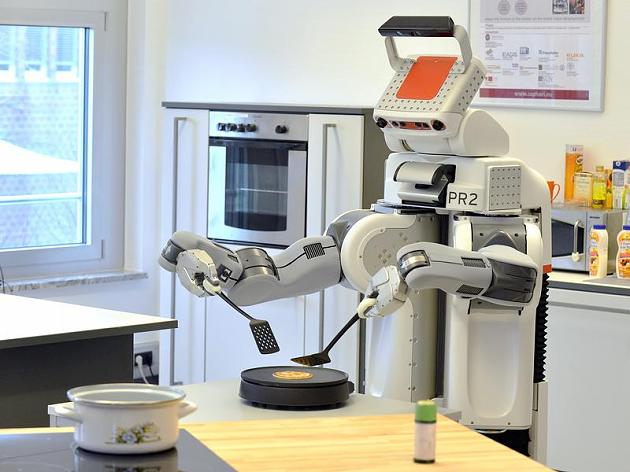
\includegraphics[scale=.25]{img/pr2.jpg}\footnote{\tiny{\url{Source: https://www.focus.de/digital/handy/technik-roboter-pr2-kann-popcorn-oder-pfannkuchen-machen\_aid\_929326.html} last viewed: 11.12.2018}}
	\end{figure}
	\begin{itemize}
		\item perception component
			\begin{itemize}
				\item detect objects
				\item analyse objects
			\end{itemize}
		\item reasoning component
			\begin{itemize}
				\item identify/classify objects based on their visual cues
				\item needs to be trained
			\end{itemize}
	\end{itemize}
\end{frame}

\begin{frame}{Creation of Training Data}
time and resource intensive:
	\begin{itemize}
		\item manually creating scenarios and images
		\item no groundtruth
	\end{itemize}
	
$\rightarrow$ synthetic images from a game engine
\end{frame}

\begin{frame}{System Setup}
	\begin{itemize}
		\item list of objects, classes and scenarios
			\begin{itemize}
				\item 43 objects
				\item 20 classes
				\item 3 scenarios (breakfast, cooking, fridge)
			\end{itemize}
		\item \textsc{Unreal Engine} to create \textit{Unreal Images}
		\item \textsc{RoboSherlock} analysis the images
		\item learn a \textit{Markov Logic Network} 
		\item classify the objects in the images
	\end{itemize}
\end{frame}

\begin{frame}{Unreal Engine}
	\begin{figure}
		
\includegraphics[scale=.15]{img/Unreal_Engine_Horiz_Black.png}
	\end{figure}	
	\begin{itemize}
		\item photorealism
		\item rendering in realtime
		\item open source
	\end{itemize}
\end{frame}

\begin{frame}{Unreal Images}
	\begin{itemize}
		\item Assets
			\begin{itemize}
				\item scanned 3D-models of the objects
				\item kitchen environment
			\end{itemize}
		\item URoboVision plugin
			\begin{itemize}
				\item create RGBD image from a scene
				\item create \textit{ObjectImage} and  \textit{ObjectMap} 
				\item send them to \textsc{RoboSherlock}
			\end{itemize}
		\item RSpawnBox class
			\begin{itemize}
				\item visual representation of scene space
				\item rotates camera around the scene
			\end{itemize}
	\end{itemize}
\end{frame}

\begin{frame}{Unreal Images}
	\begin{itemize}
		\item 114 scenes
		\item 2 - 5 objects per scene
		\item 5 viewpoints per scene
		\item only objects of one scenario per scene
		\item total of 570 images
	\end{itemize}
	\begin{figure}
\centering
	\begin{subfigure}[b]{0.3\textwidth}
		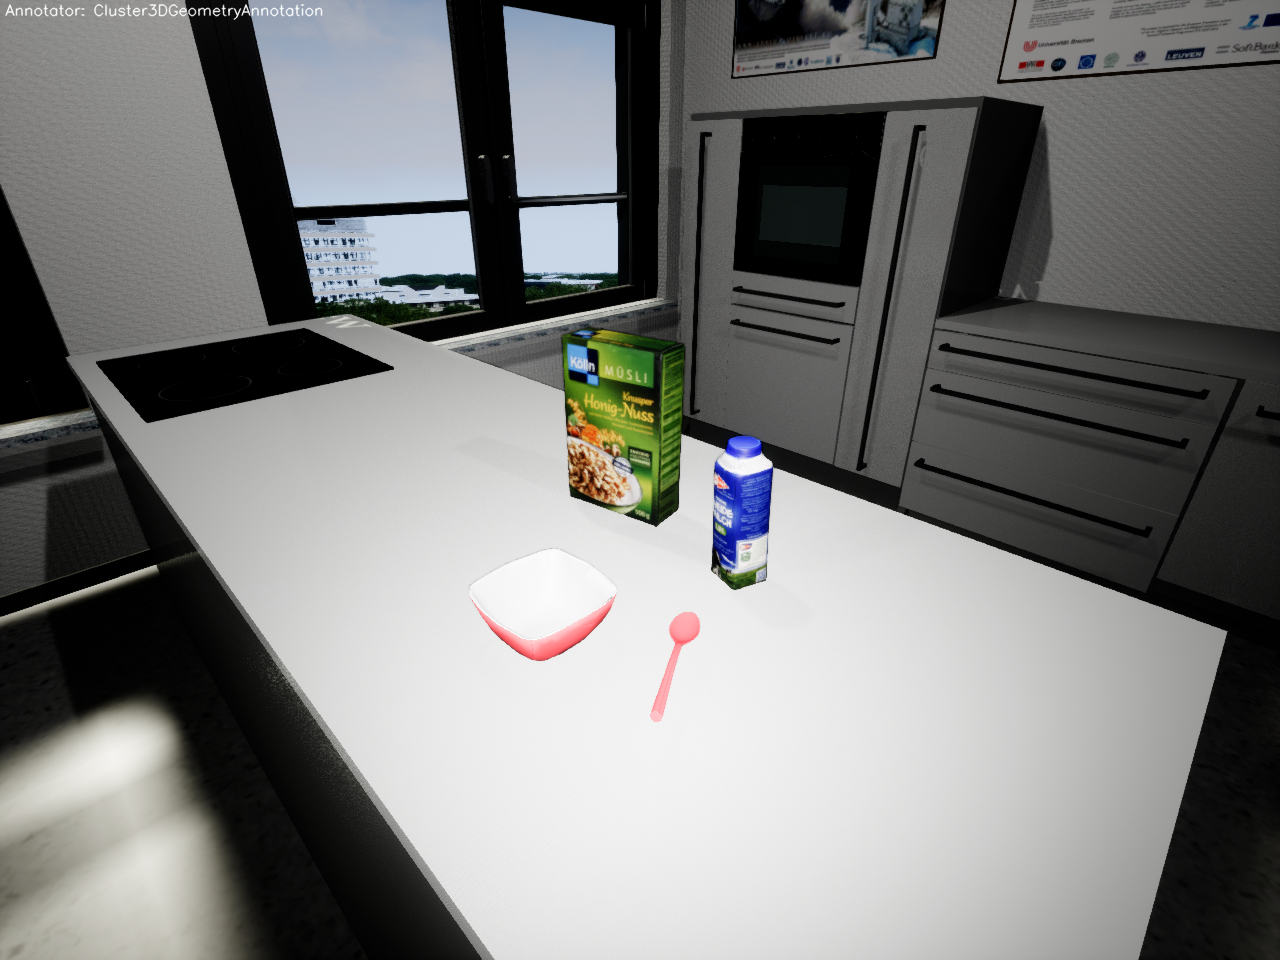
\includegraphics[scale=.07]{../thesis/img/chapter3/sceneEx_1}
	\end{subfigure}
	\quad
	\begin{subfigure}[b]{0.3\textwidth}
		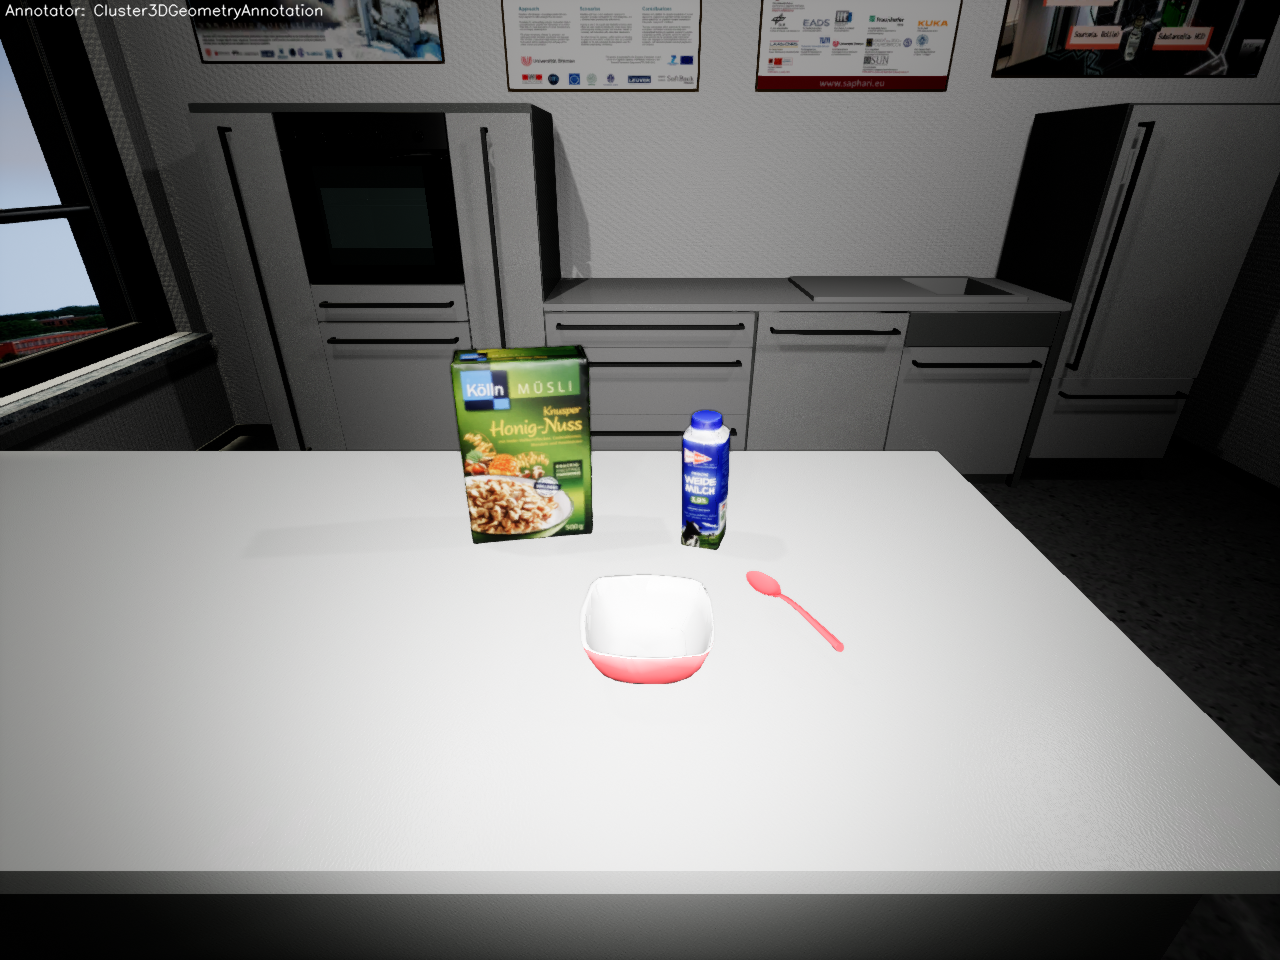
\includegraphics[scale=.07]{../thesis/img/chapter3/sceneEx_2}	
	\end{subfigure}
	\quad
	\begin{subfigure}[b]{0.3\textwidth}
		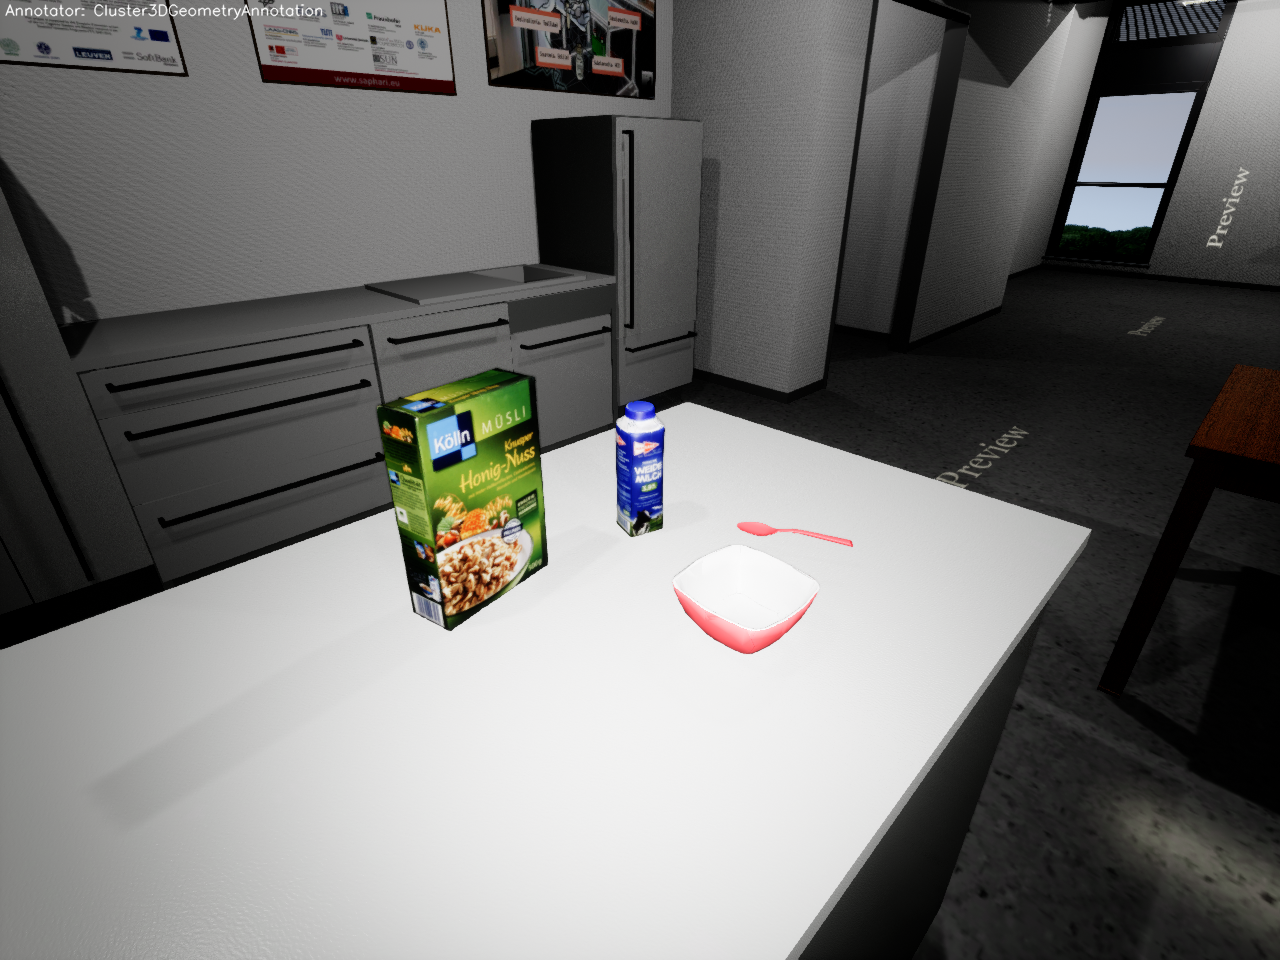
\includegraphics[scale=.07]{../thesis/img/chapter3/sceneEx_3}	
	\end{subfigure}
	\quad
	\begin{subfigure}[b]{0.3\textwidth}
		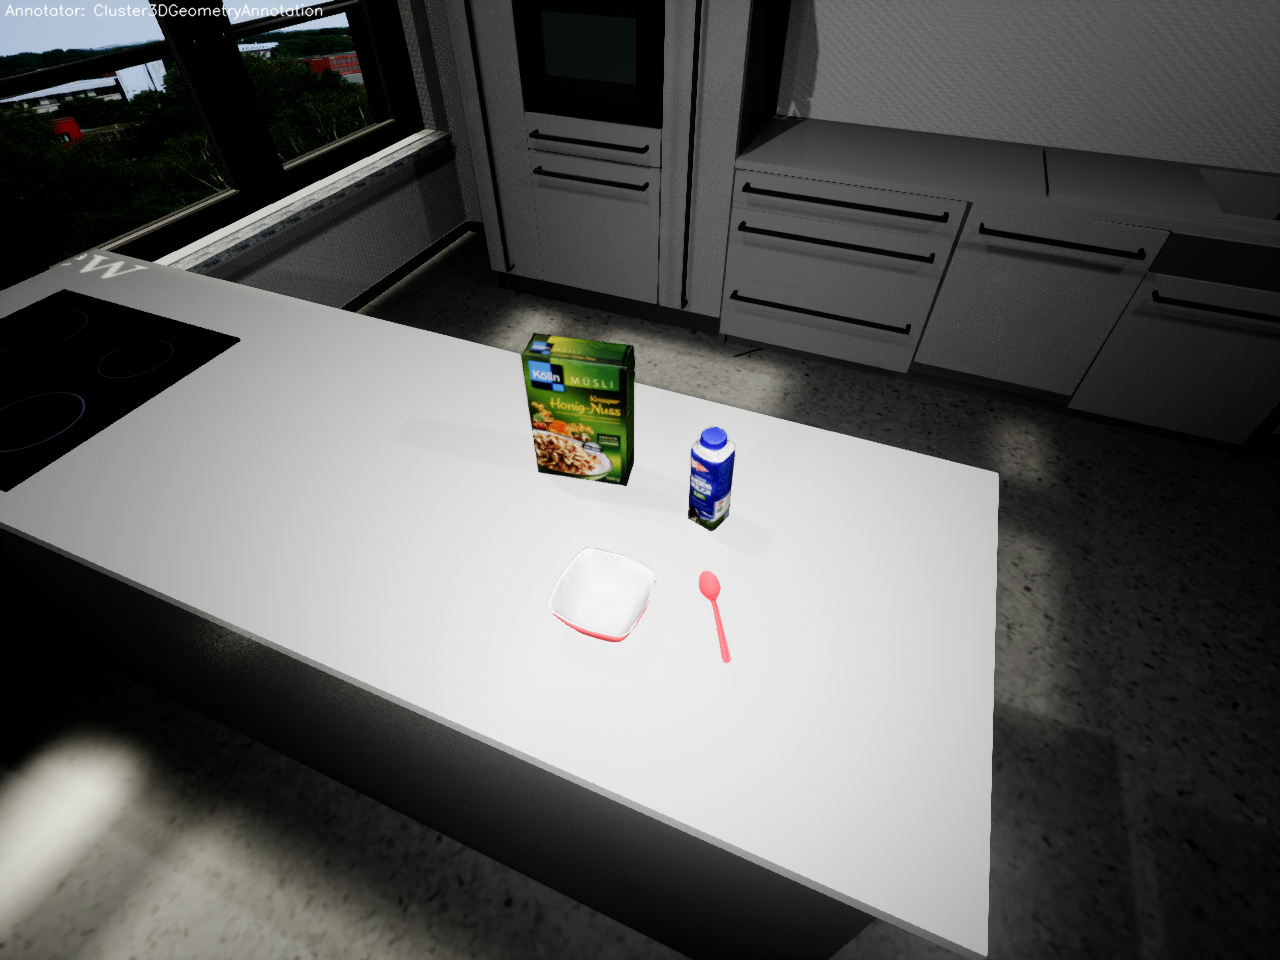
\includegraphics[scale=.07]{../thesis/img/chapter3/sceneEx_4}	
	\end{subfigure}
	\quad
	\begin{subfigure}[b]{0.3\textwidth}
		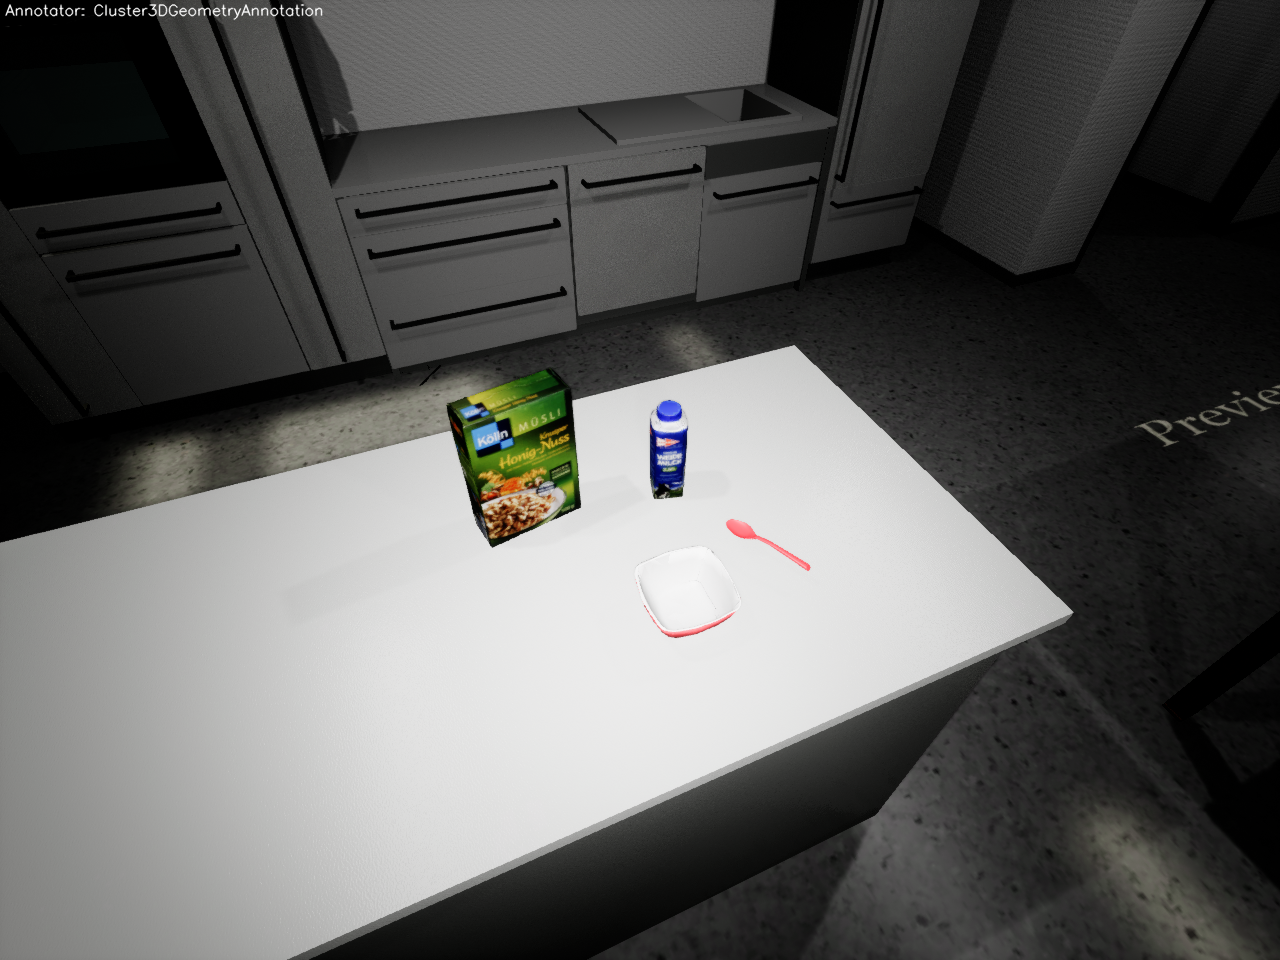
\includegraphics[scale=.07]{../thesis/img/chapter3/sceneEx_5}	
	\end{subfigure}
\end{figure}
\end{frame}


\begin{frame}{RoboSherlock}
	\begin{figure}
		
\includegraphics[scale=.3]{img/rs_logo_text.png}
	\end{figure}
	\begin{itemize}
		\item based on \textit{UIMA}
		\item segments images and creates object hypotheses
		\item annotates attributes of the hypotheses
	\end{itemize}	
\end{frame}

\begin{frame}{Perceptionpipeline}
Annotates the following attributes:
	\begin{itemize}
		\item color
		\item size
		\item shape
		\item goggles\_\{Logo, Text, Product\}
		\item instance
		\item object
	\end{itemize}
\end{frame}

\begin{frame}{UnrealGTAnnotator}
Annotates the groundtruth by:
	\begin{itemize}
		\item counting the color of pixels in the ObjectImage
		\item looking up the corresponding asset 
		\item looking up the groundtruth for that asset
		\item setting the groundtruth 
	\end{itemize}

\end{frame}


\begin{frame}{Markov Logic Networks}
	\begin{itemize}
		\item consists of formulas and real-valued weights
		\item describes a \textit{Markov Network} with a joint probability distribution
		\item is able to:
		\begin{itemize}
			\item model relations between objects
			\item compensate inconsistencies
			\item reason about every aspect represented in the model
		\end{itemize}
		\item used Toolbox: \textsc{pracmln}
	\end{itemize}
\end{frame}

\begin{frame}{PR2 Looking at Things}
Experiments:
	\begin{itemize}
		\item \textsc{RoboSherlock} + MLNs
		\item 50 images 
		\item 21 object categories
		\item 4 scenarios
	\end{itemize}
\bigskip
Results:
	\begin{itemize}
		\item Annotators are complementary
		\item classification rate of 69\%
	\end{itemize}
\end{frame}

\begin{frame}{Experiments}
	\begin{itemize}
		\item instance and class classification
		\item 10 fold cross validation for Unreal Images
		\item Unreal Images for Training, Real Images for Testing
		\item mixed trainingset
	\end{itemize}
\end{frame}

\begin{frame}{Experiments - MLN model}
\begin{align*}
& w_{1} \ shape(?c, +?sha) \wedge object(?c, +?obj) \\
& w_{2} \ color(?c, +?col) \wedge object(?c, +?obj) \\
& w_{3} \ size(?c, +?size) \wedge object(?c, +?obj) \\
& w_{4} \ instance(?c, +?inst) \wedge object(?c, +?obj) \\
& w_{5} \ goggles\_Logo(?c, +?comp) \wedge object(?c, +?obj)\\
& w_{6} \ goggles\_Text(?c, +?text) \wedge object(?c, +?obj)\\
& w_{7} \ goggles\_Product(?c, +?prod) \wedge object(?c, +?obj)\\
& w_{8} \ scene(+?s) \wedge object(?c, +?obj)\\
& w_{9} \ object(?c1, +?t1) \wedge object(?c2, +?t2) \wedge ?c1 =/= ?c2
\end{align*}

\end{frame}

\begin{frame}{Experiments - 10 fold cross validation}
\begin{columns}
	\begin{column}{0.7\textwidth}
		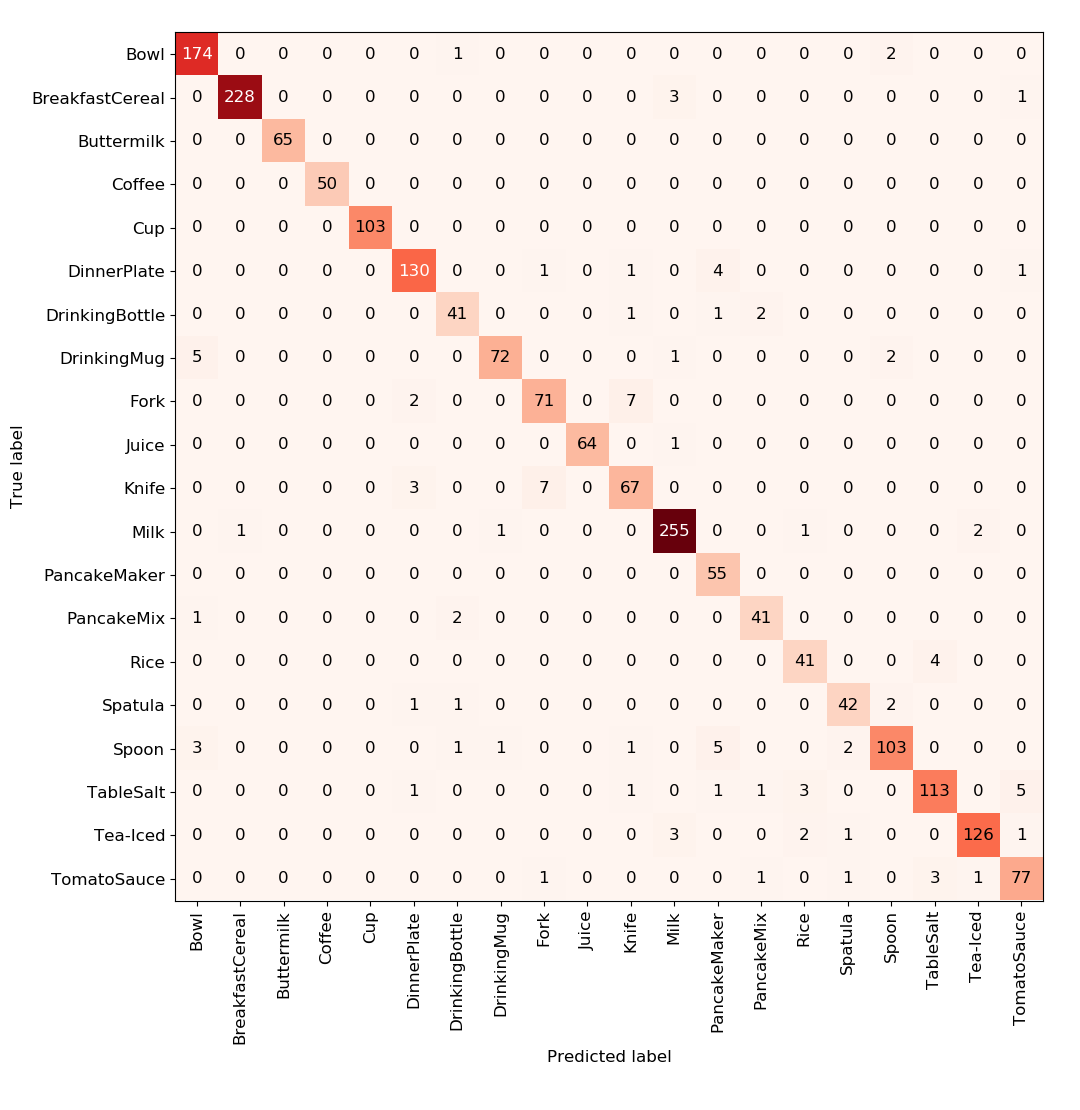
\includegraphics[scale=.3]{../thesis/img/chapter6/UnrealGTClass.png}
	\end{column}
	\quad
	\begin{column}{0.3\textwidth}
		\begin{itemize}
			\item Accuracy: 95\%
			\item Precision: 95\%
			\item Recall: 95\%
			\item F$_{1}$-Score: 95\%
			\bigskip
			\item Instance scores: 96\%
		\end{itemize}
	\end{column}
\end{columns}
\end{frame}

\begin{frame}{Experiments - Complementary Experts}
\begin{columns}
	\begin{column}{0.5\textwidth}
		\begin{figure}
			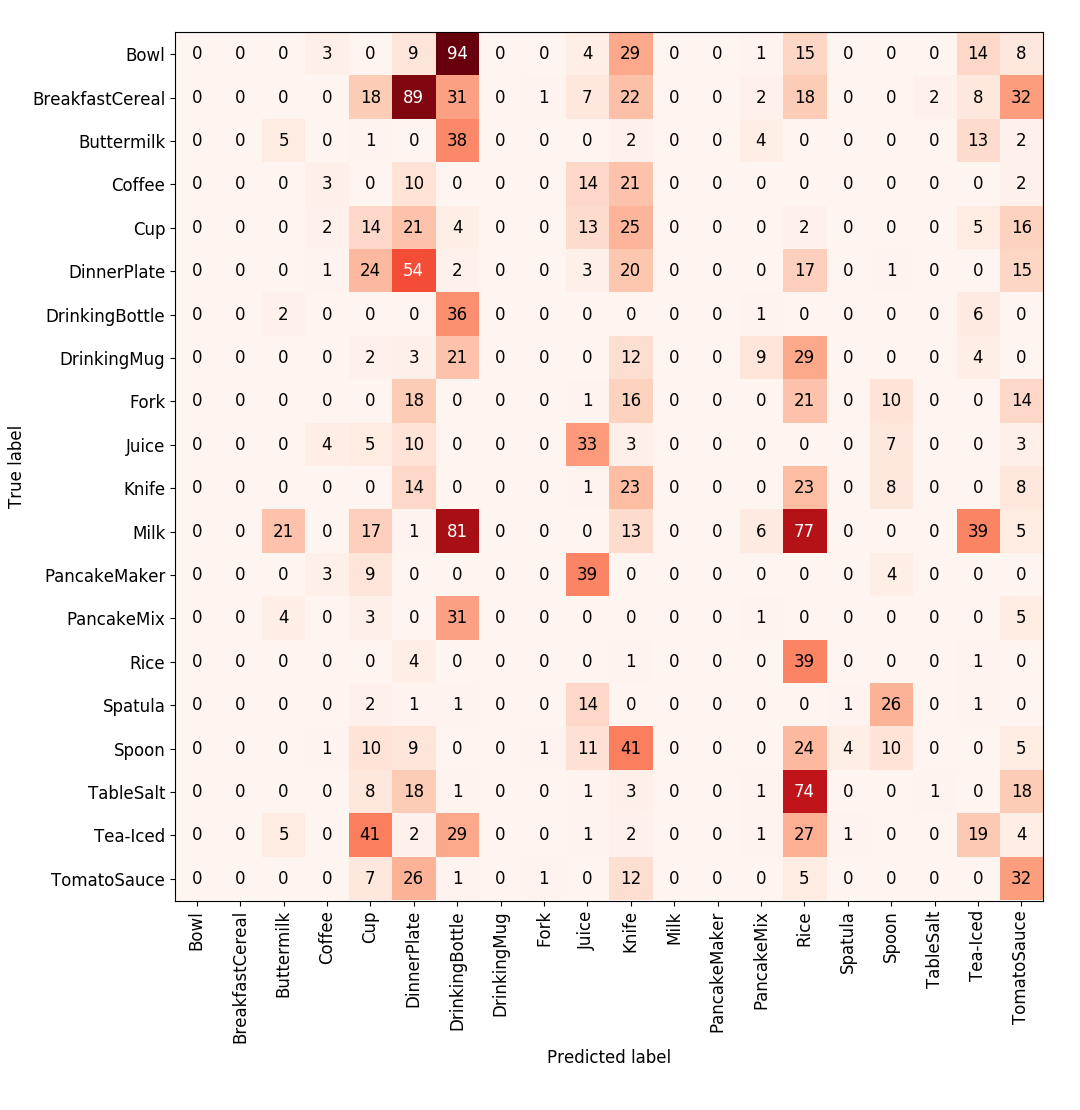
\includegraphics[scale=.2]{../thesis/img/chapter6/UnrealGTClass_color.png}
			\caption{color}
		\end{figure}	
	\end{column}
	\quad
	\begin{column}{0.5\textwidth}
		\begin{figure}
			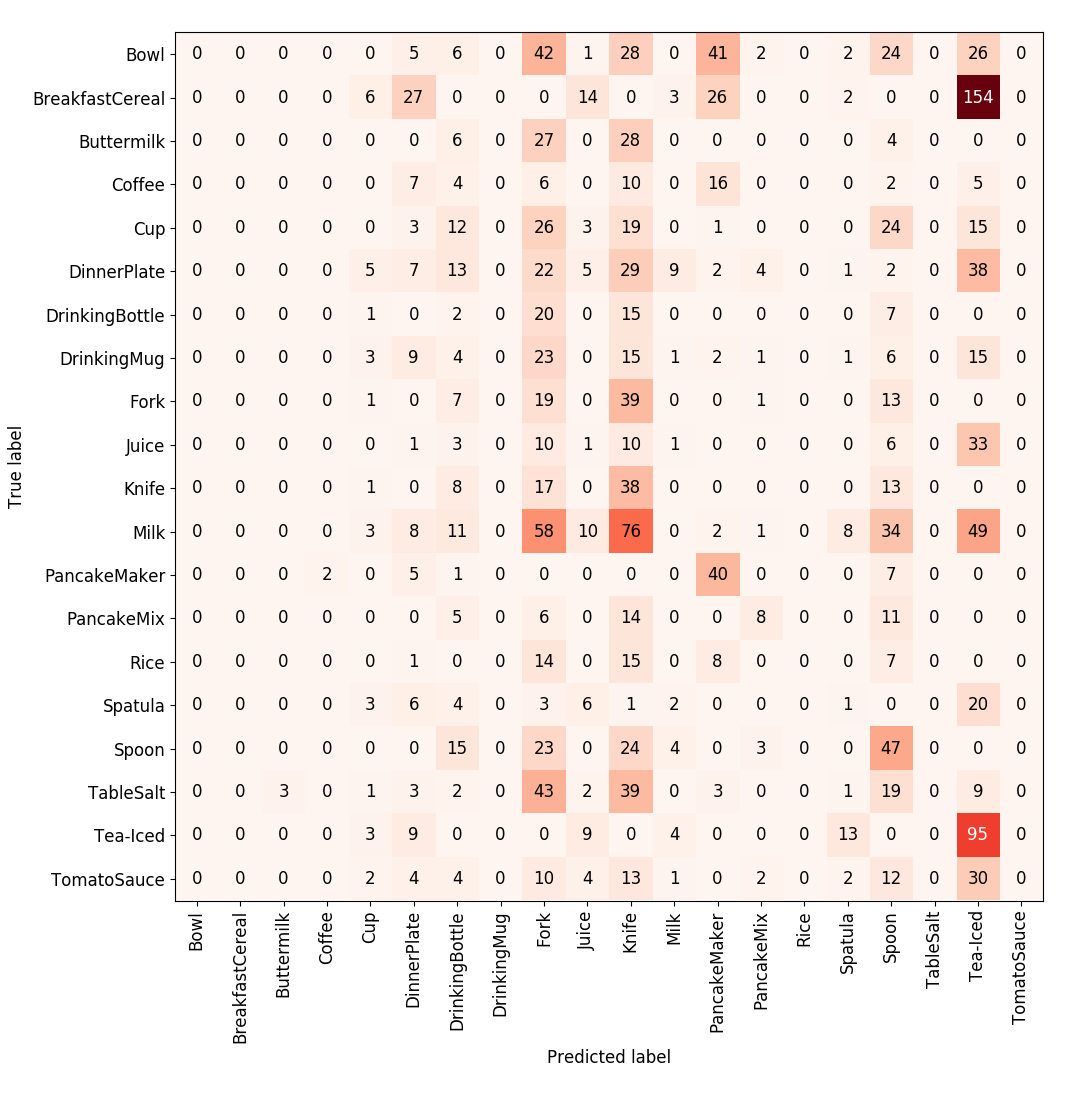
\includegraphics[scale=.2]{../thesis/img/chapter6/UnrealGTClass_size.png}
			\caption{size}
		\end{figure}
	\end{column}
\end{columns}
\end{frame}

\begin{frame}{Experiments - Complementary Experts}
\begin{columns}
	\begin{column}{0.5\textwidth}
		\begin{figure}
			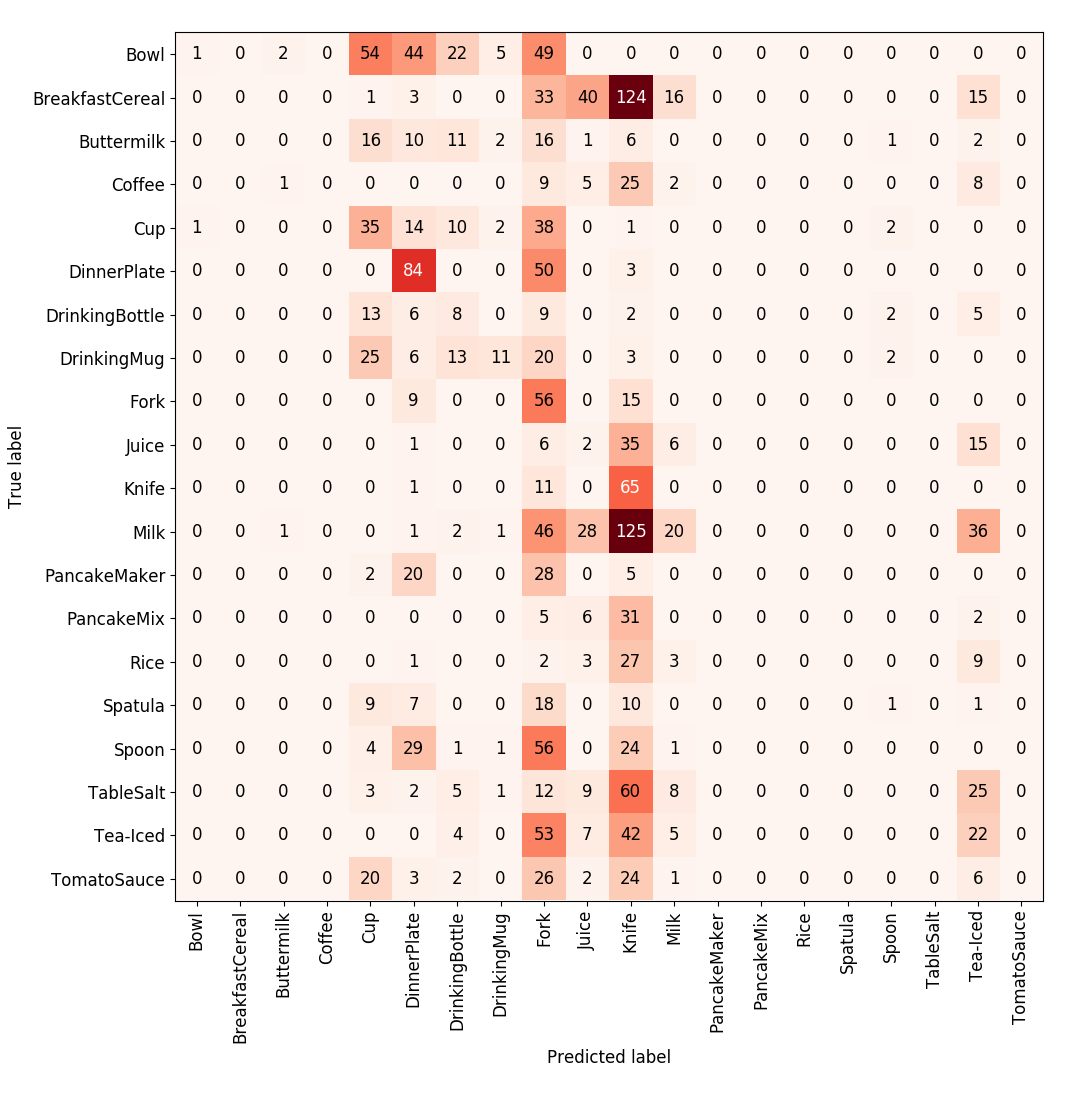
\includegraphics[scale=.2]{../thesis/img/chapter6/UnrealGTClass_shape.png}
			\caption{shape}
		\end{figure}	
	\end{column}
	\quad
	\begin{column}{0.5\textwidth}
		\begin{figure}
			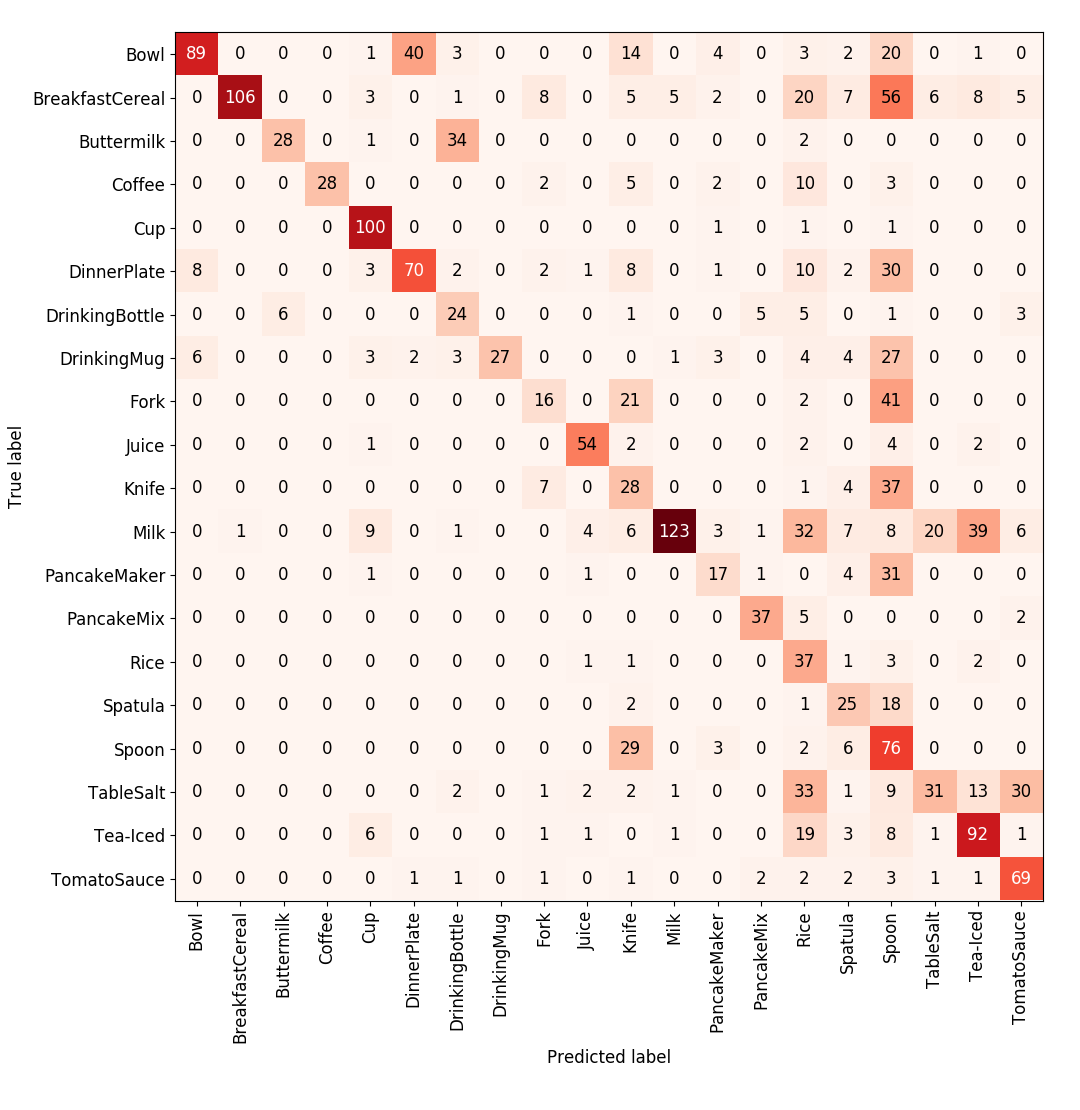
\includegraphics[scale=.2]{../thesis/img/chapter6/UnrealGTClass_instance.png}
			\caption{instance}
		\end{figure}
	\end{column}
\end{columns}
\end{frame}

\begin{frame}{Experiments - Testing with Real Images}
\begin{columns}
	\begin{column}{0.7\textwidth}
		\includegraphics[scale=.3]{../thesis/img/chapter6/UnrealRealGTClass.png}
	\end{column}
	\quad
	\begin{column}{0.3\textwidth}
		\begin{itemize}
			\item Accuracy: 76\%
			\item Precision: 78\%
			\item Recall: 76\%
			\item F$_{1}$-Score: 76\%
			\bigskip
			\item Instance scores:
			\begin{itemize}
				\item Accuracy: 66\%
				\item F$_{1}$-Score: 65\%
			\end{itemize}
		\end{itemize}
	\end{column}
\end{columns}
\end{frame}

\begin{frame}{Experiments - Mixed Trainingset}
\begin{columns}
	\begin{column}{0.7\textwidth}
		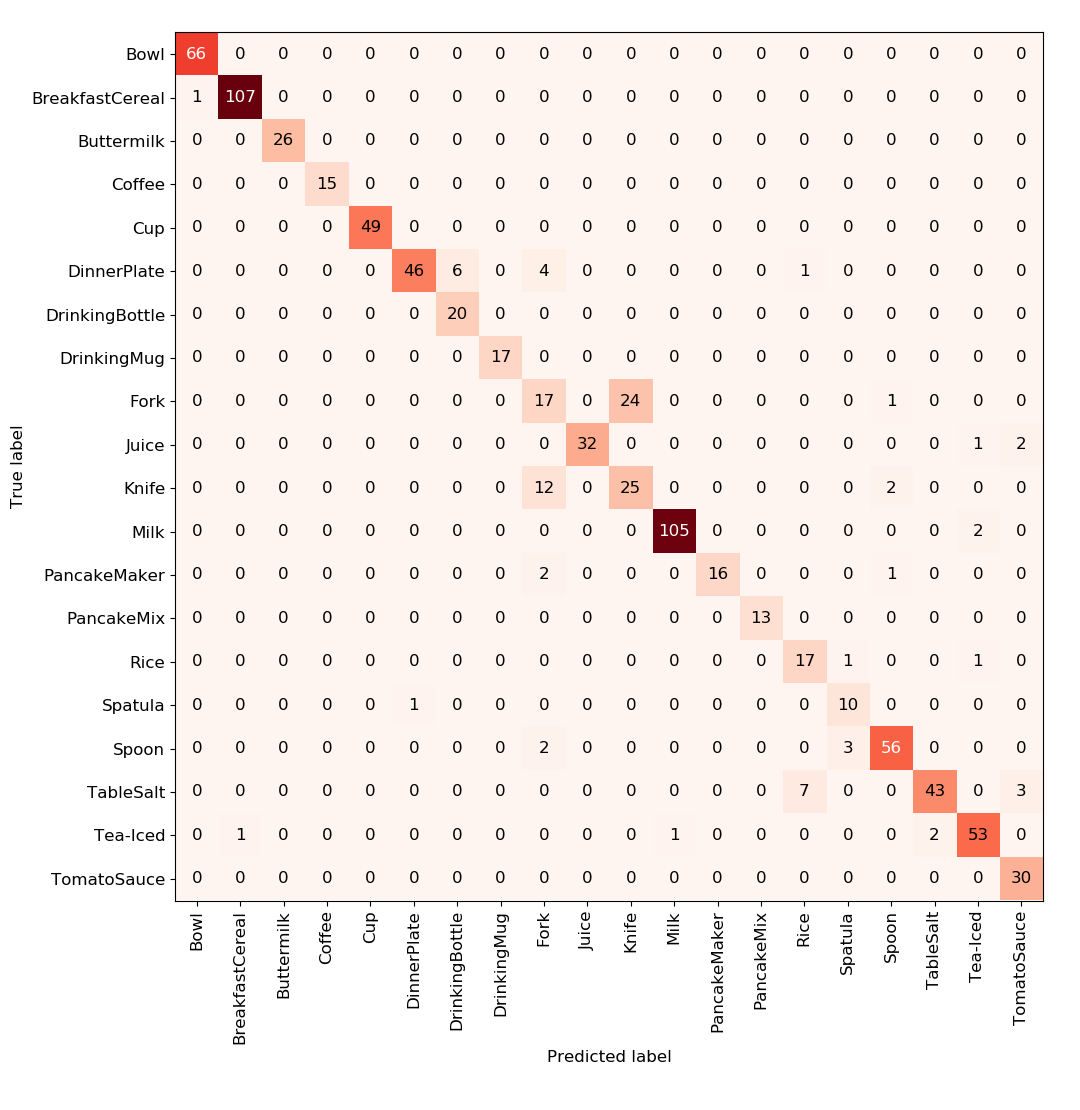
\includegraphics[scale=.3]{../thesis/img/chapter6/UnrealRealMixedGTClass.png}
	\end{column}
	\quad
	\begin{column}{0.3\textwidth}
		\begin{itemize}
			\item Accuracy: 90\%
			\item Precision: 91\%
			\item Recall: 90\%
			\item F$_{1}$-Score: 90\%
			\bigskip
			\item Instance scores: 88\%
		\end{itemize}
	\end{column}
\end{columns}
\end{frame}

\begin{frame}{Conclusion}
	\begin{itemize}
		\item Unreal Images can be used for training
		\item complementary nature of MLNs is applicable 
		\item mixed trainingsets can boost performance
		\bigskip
		\item automation of training data creation is possible
	\end{itemize}
\end{frame}

\end{document}

